\chapter{Experiments and Applications}

In the previous two chapters the mathematical and computational challenges of image reconstruction for CT have been discussed. In chapter 3, a detailed description of a variety of different algorithms has been presented, including the ART family of algorithms, CGLS, MLEM and few TV approaches for smooth reconstruction, as well as the classic FDK reconstruction. Additionally in chapter 4 the computational aspect of CT is discussed, on where the problems computing the exact adjoint of the projection operation and mainly the computational burden of some of the operations have been mentioned. Considering the variety of available methods and the specifics of the implementation of the software developed, the TIGRE toolbox, experiments on how these algorithms compare and behave are due. Further than that, the performance of these algorithm in different experimental datasets is also an important analysis.

This chapter shows experimental analysis on both of the topics. First a variety of convergence analysis with different algorithms using synthetic data are performed, showing the differences not only between algorithms, but also between option on parameter selections. The section tries to illustrate and perhaps help build intuition on all the different parameters and options that each of these algorithms has, both within the algorithms themselves and among the different ones. Additionally some highlights on the practical challenges that the use of the algorithms entail in real applications are given.

In the second section of this chapter, a few examples of some of the algorithms are shown in different CT applications, both cone and parallel beam. Data from various different applications, from medicine to science has been tested using the TIGRE toolbox. While quantitative analysis is not possible with these datasets because the truth is not known, some insight in how the algorithms behave in each case is discussed.

\section{Algorithm Experiments}

\begin{figure}
\begin{center}

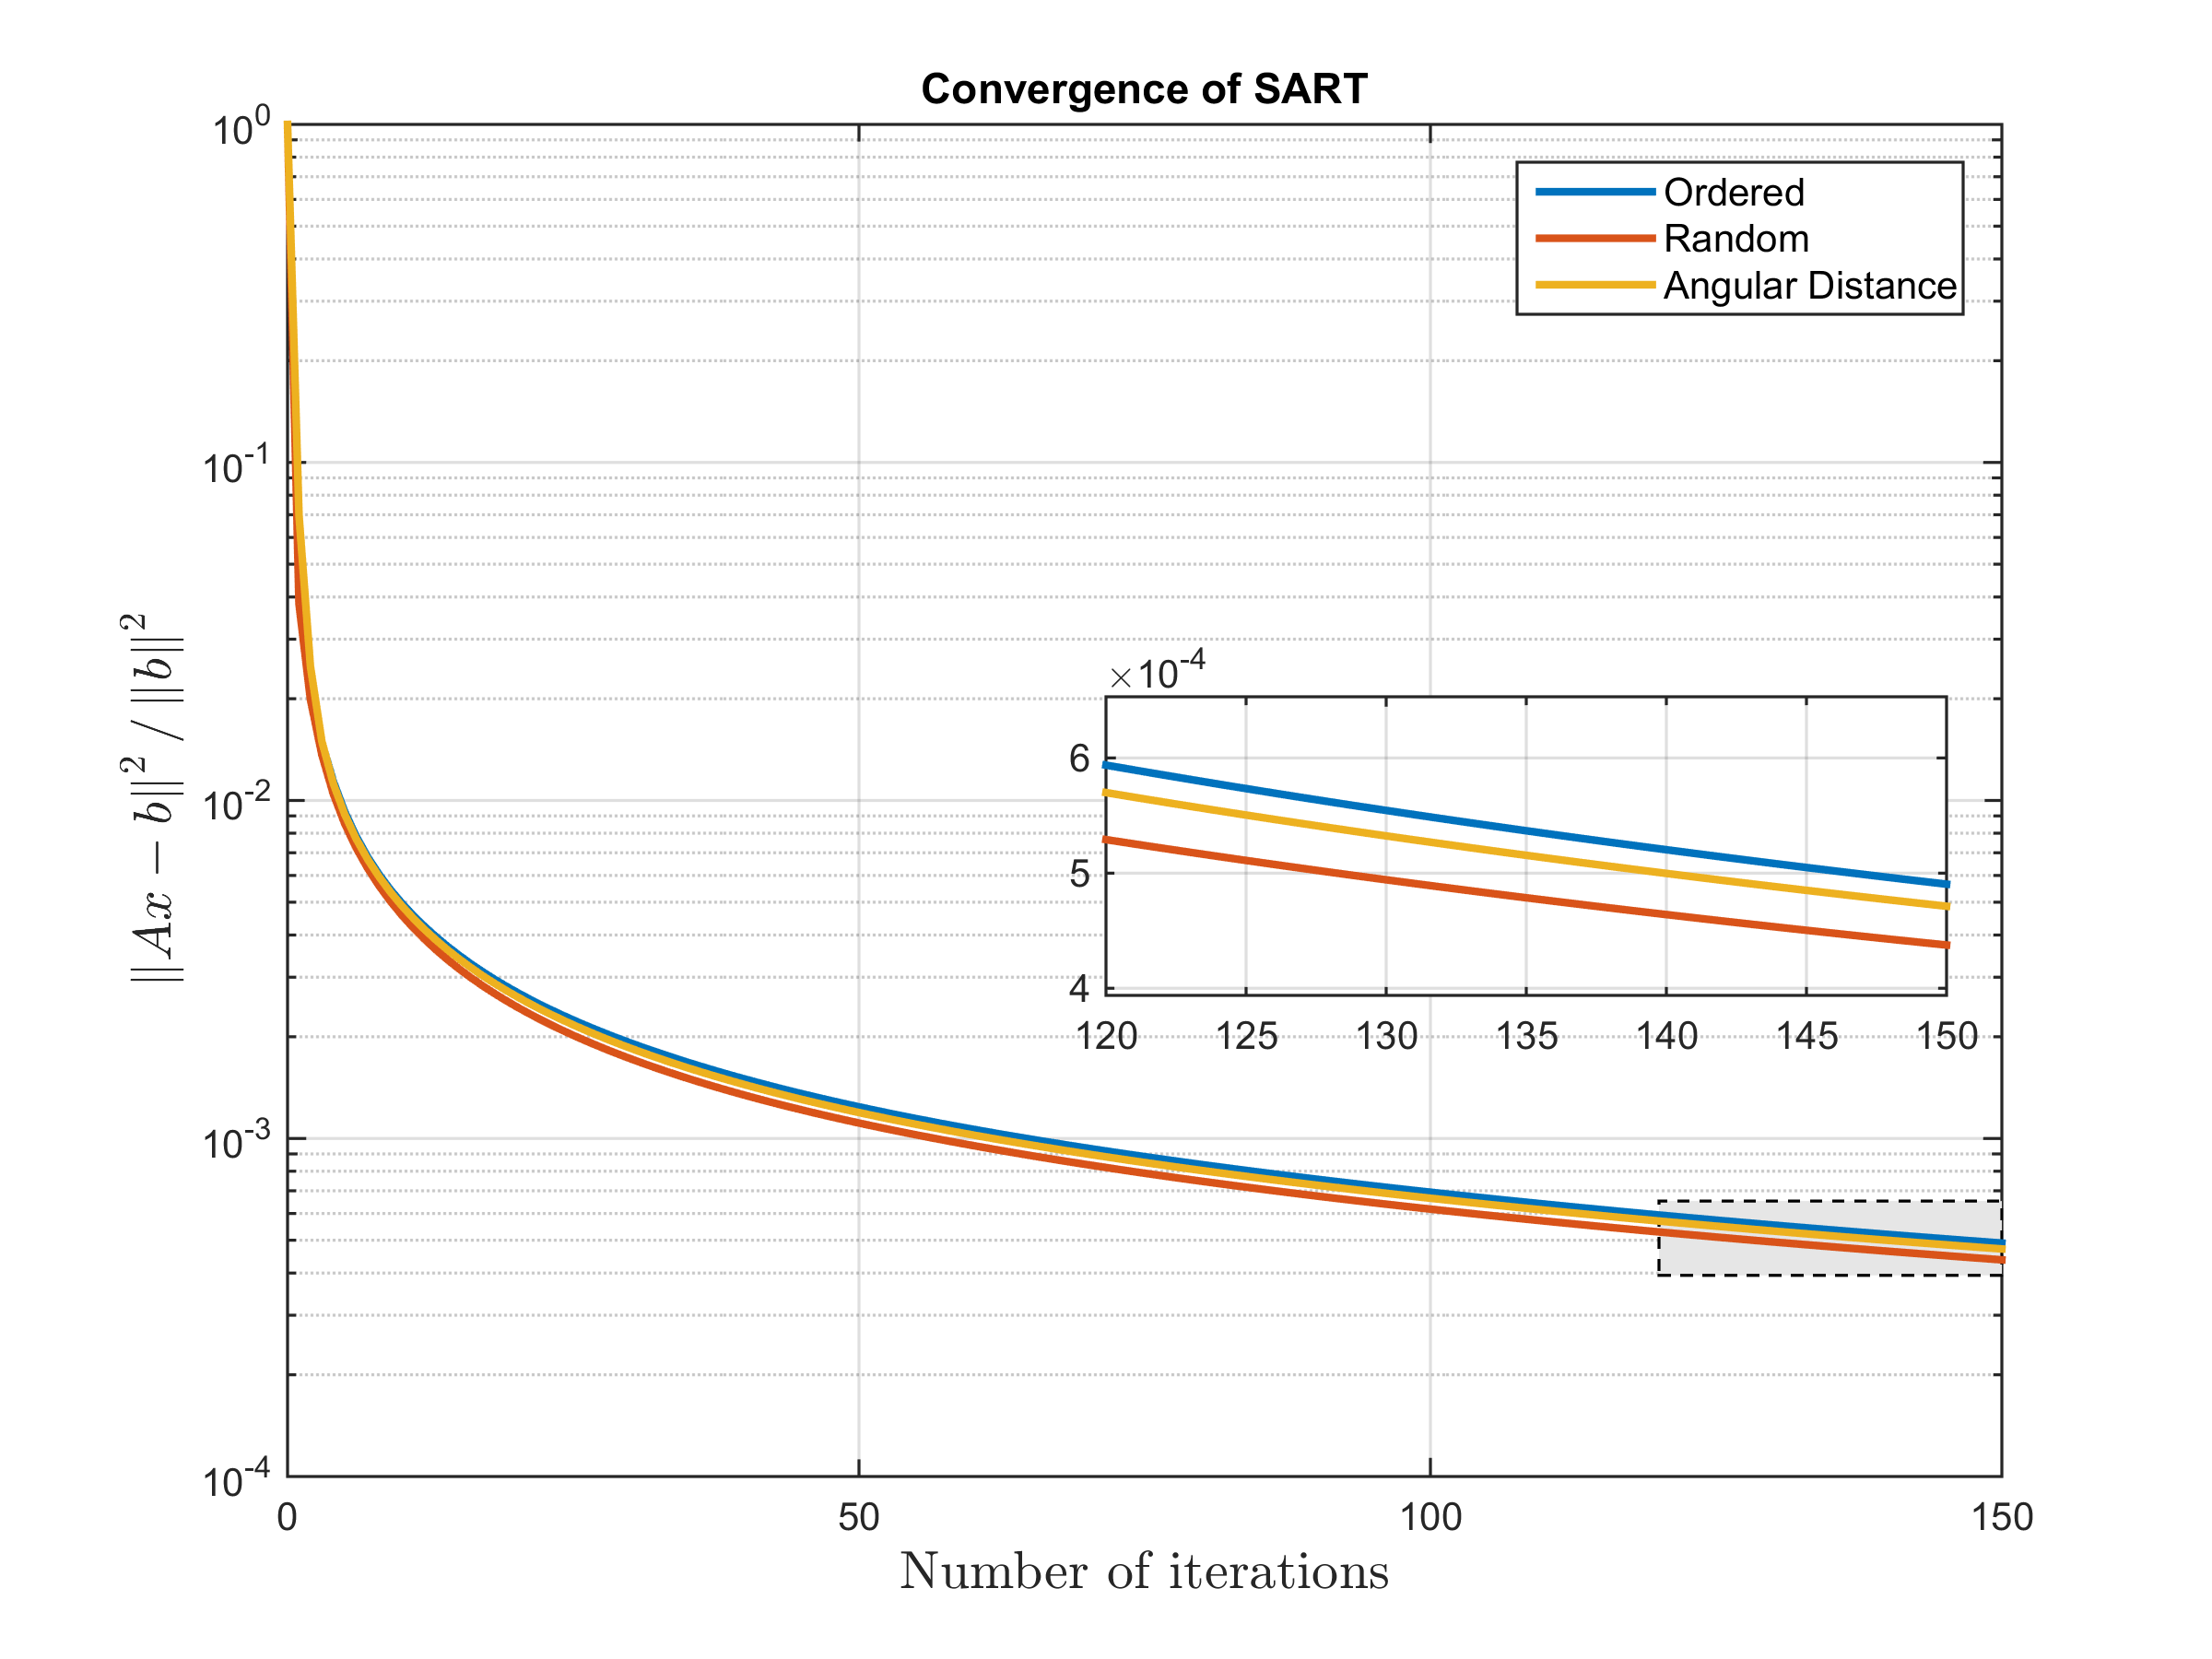
\includegraphics[width=0.9\textwidth]{Applications/SARTangles.png} 
\end{center}

\caption[qewqwe]{\label{fig:wqe} qweqwe.} 
\end{figure}

\section{Iterative Algorithms in Different CT Applications}
\subsection{Medical Head CBCT from  The Christie Hospital}
\subsection{Cryo Soft X-Ray Tomography at Diamond Light Source}